%/**************************************
% * Displaying Wind Vectors in ArcGIS Pro  *
%/**************************************
\documentclass[12pt]{article}
%\documentstyle{report}
\usepackage{float}
\usepackage{graphicx}
\usepackage[margin=1in]{geometry}
%\usepackage{subfig}


\graphicspath{{images/}}

\usepackage[utf8]{inputenc}
\usepackage[english]{babel}
\usepackage[parfill]{parskip}
\usepackage{datetime}
\usepackage{hyperref}
\hypersetup{
	colorlinks=true,
	urlcolor=blue,
  }
\urlstyle{same}
%\newdate{date}{26}{04}{2018}
%\date{\displaydate{date}}
%\usepackage{subcaption} 
\usepackage{subfig}
\usepackage{dirtytalk}
\usepackage{multirow}
\usepackage{booktabs}
\usepackage{enumitem}
\usepackage{nameref}

\usepackage{fancyhdr}
\pagestyle{fancy}
\fancyhf{}
\rhead{Displaying and Rotating WindNinja-Derived
Wind Vectors in ArcGIS Pro 3.3.1}
\setlength{\headheight}{14.49998pt}
\cfoot{\thepage}

\newcommand\vn{3.6.0}

\begin{document}
\begin{titlepage}
    \centering
    {\Huge
        Displaying and Rotating WindNinja-Derived Wind Vectors in ArcGIS Pro 3.3.1
    }
    \vfill
    {\Large
    Gabriel Abreu Vigil\\ RMRS, Fire Sciences Lab, Missoula, MT, \href{mailto:gabriel.abreuvigil@usda.gov}{gabriel.abreuvigil@usda.gov}

    Mason Willman\\ RMRS, Fire Sciences Lab, Missoula, MT, \href{mailto:mason.willman@usda.gov}{mason.willman@usda.gov}

    Chuck McHugh\\ RMRS, Fire Sciences Lab, Missoula, MT, 406-829-6953, \href{mailto:cmchugh@fs.fed.us}{cmchugh@fs.fed.us}
    }
    \vfill
    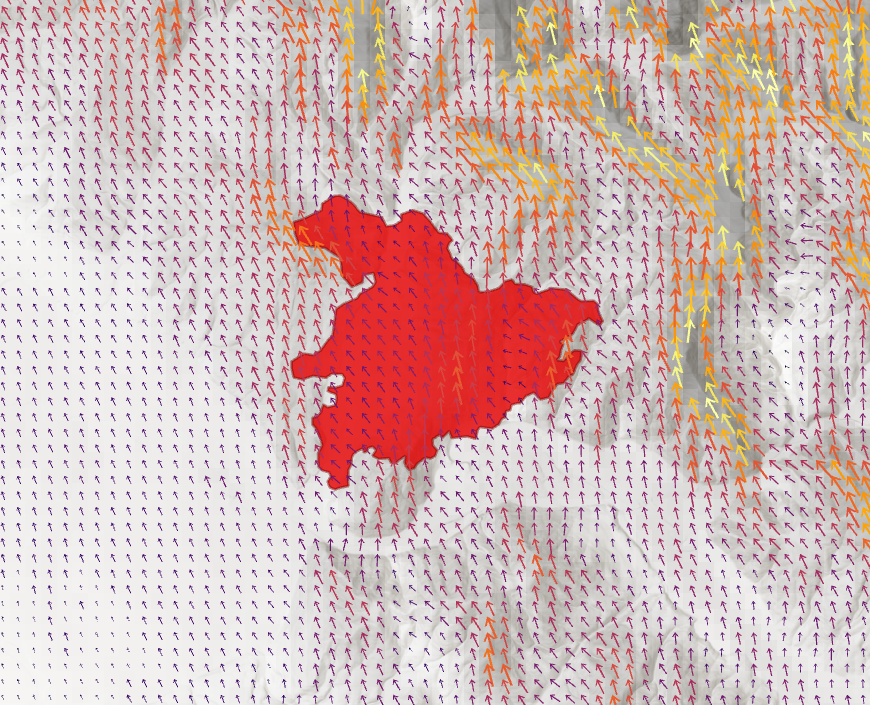
\includegraphics[scale=0.7]							{arc_00.png}
    \vfill
  	{\Large
	  01/30/2025 %Date Last Edited
  	}
    \vfill
\end{titlepage}

\section*{Displaying WindNinja-generated gridded wind vectors}
Data requirements are a Shapefile Feature Class format. The shapefile generated during the WindNinja process will
contain five data fields in the associated .DBF file (Figure \ref{fig:Figure1}).

\begin{figure}[H]
	\centering
	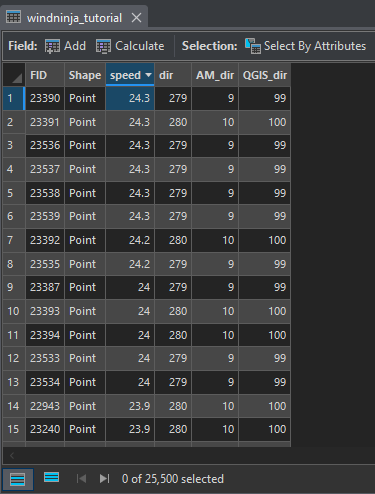
\includegraphics[scale=0.9]{arc_1.png}
	\caption{Attribute table for WindNinja-generated shapefile as displayed in ArcGIS Pro.}
	\label{fig:Figure1}
\end{figure}

\begin{enumerate}[label=(\alph*)]
\item \textbf{FID:} Feature ID, a unique number assigned to that point by ArcGIS Pro.
\item \textbf{Shape:} Point indicates that the feature type for the shapefile is a point
\item \textbf{speed:} WindNinja-generated wind speed at the specified output height and in the specified output units.
\item \textbf{dir:} WindNinja-generated azimuth direction the wind is coming from in degrees (e.g., 0 degrees is wind from
the north).
\item \textbf{AM\_dir:} WindNinja-manipulated value required for use in ArcGIS Pro for display purposes.
\item \textbf{QGIS\_dir:} WindNinja-manipulated value required for use in QGIS for display purposes
\end{enumerate}
\subsection*{Steps:}
\begin{enumerate}
\item Open ArcGIS Pro and load any data coverages and fire perimeter files of interest.
\item Load the ArcGIS Pro WindNinja shapefile for the fire of interest. The wind vector grid will appear on the
coverage as individual points (Figure~\ref{fig:Figure2}).

\begin{figure}[H]
	\centering
	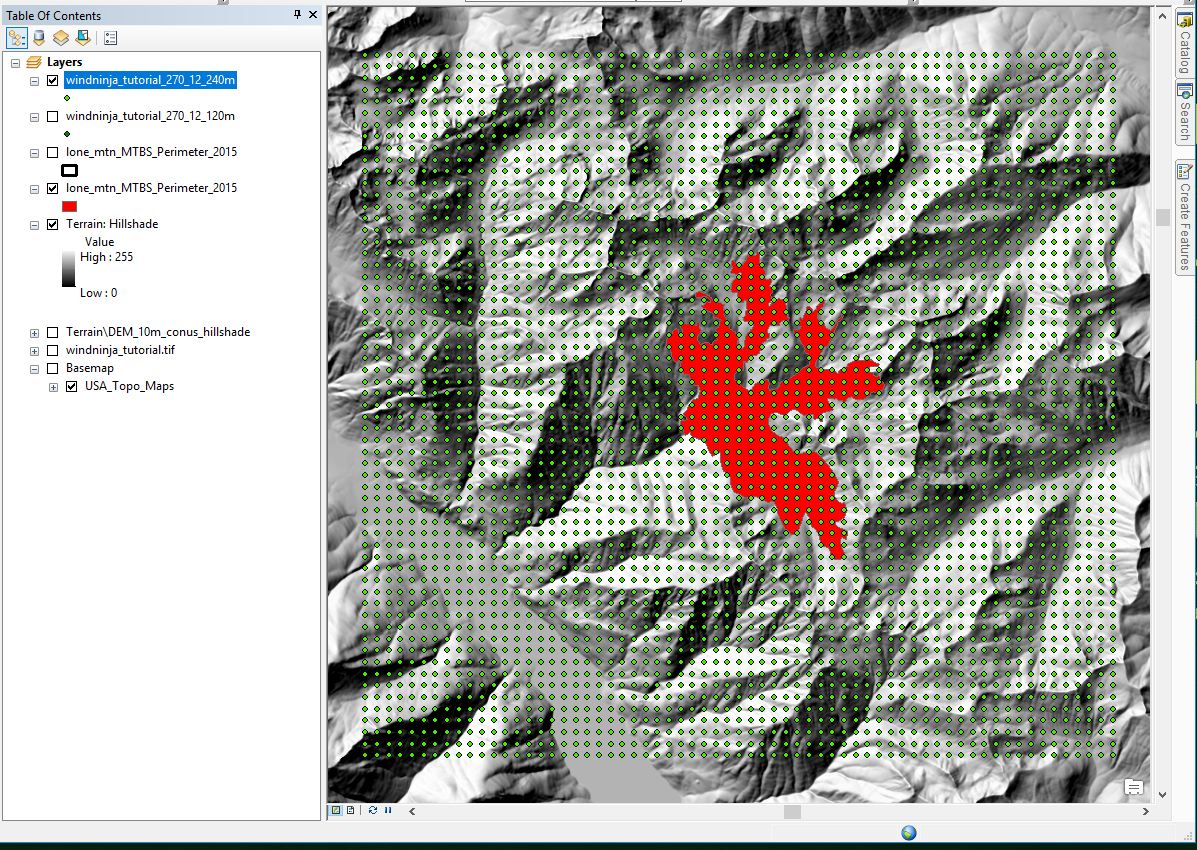
\includegraphics[scale=0.3]{arc_2.png}
	\caption{Example ArcGIS Pro project with WindNinja-generated shapefile as displayed in ArcGIS Pro prior to scaling and rotation of the
WindNinja-generated vectors.}
\label{fig:Figure2}
\end{figure}

\item After loading the file into the ArcGIS Pro project, right click on the layer name in the  \textbf{Table of Contents} then select \textbf{Symbology} (Figure~\ref{fig:Figure3}). This will open the symbology panel in (Figure~\ref{fig:Figure4}). 

\begin{figure}[H]
	\centering
	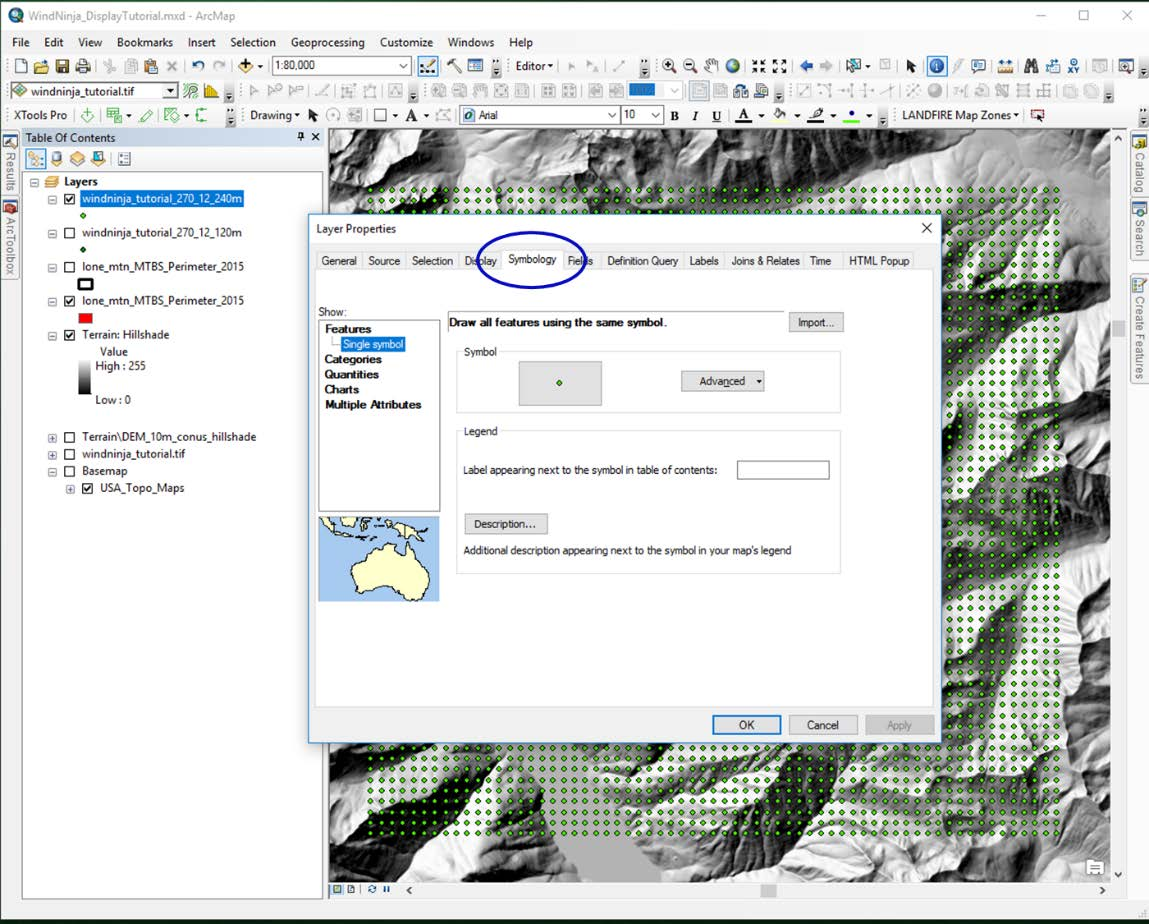
\includegraphics[scale=0.3]{arc_3.png}
	\caption{Layer Properties dialog box as displayed in ArcGIS Pro.}
\label{fig:Figure3}
\end{figure}

\begin{figure}[H]
	\centering
	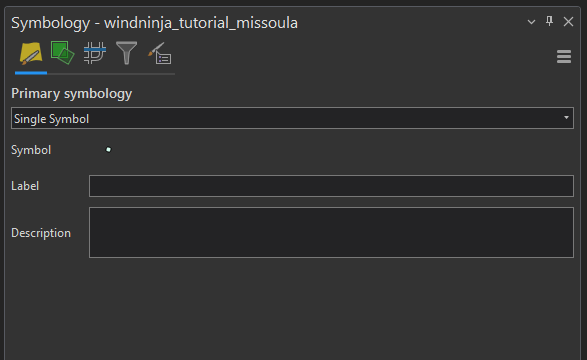
\includegraphics[scale=0.8]{arc_4.png}
	\caption{Symbology panel as displayed in ArcGIS Pro}
\label{fig:Figure4}
\end{figure}

\item Under \textbf{Primary Symbology}, select \textbf{Graduated Symbols} (Figure~\ref{fig:Figure5}).

\begin{figure}[H]
	\centering
	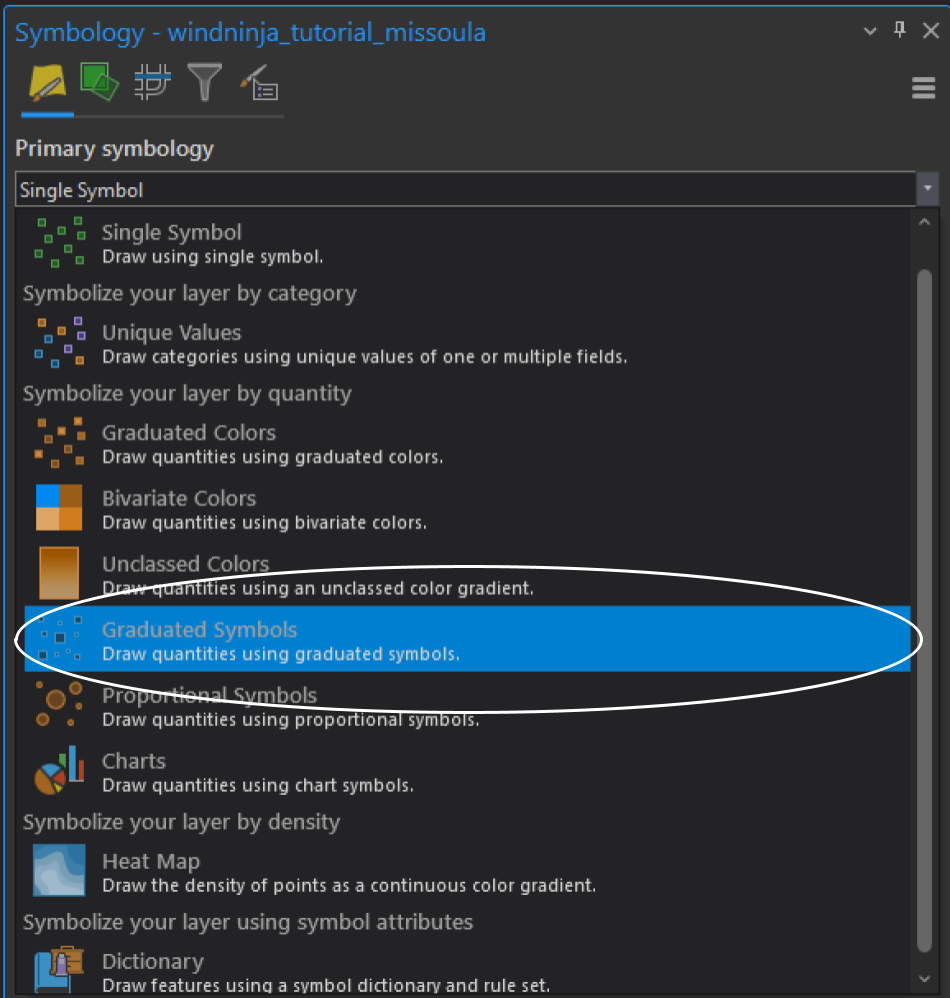
\includegraphics[scale=0.28]{arc_5.png}
	\caption{Selecting Graduated Symbols from Primary Symbology.}
\label{fig:Figure5}
\end{figure}

\item In the Field drop down, make sure that \textbf{speed} is selected from the available options. 

\begin{figure}[H]
	\centering
	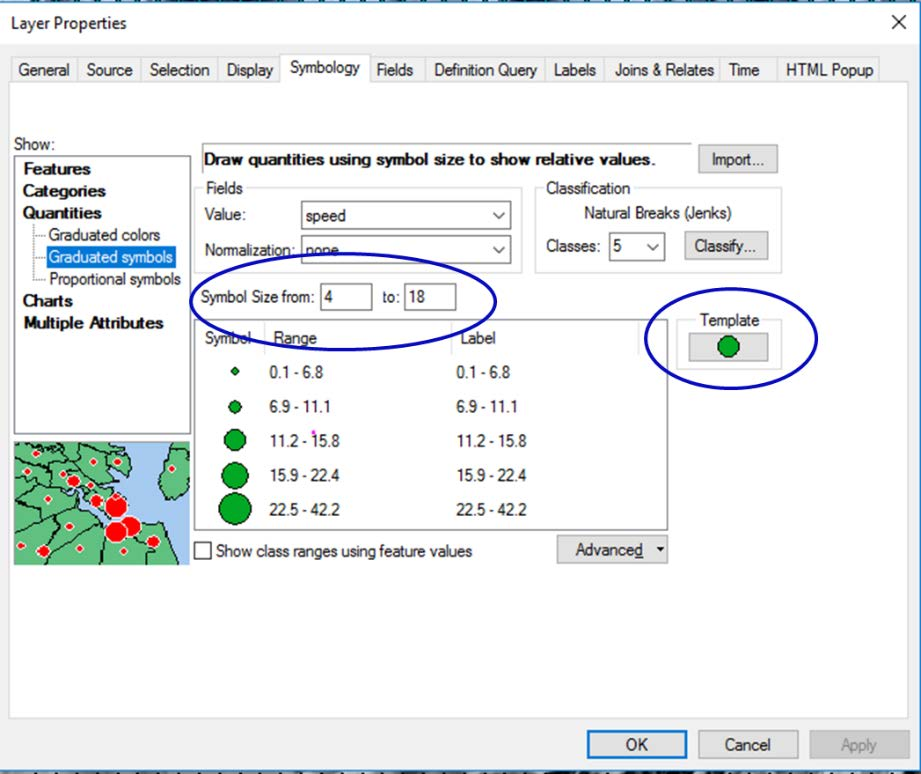
\includegraphics[scale=0.28]{arc_6.png}
	\caption{Selecting speed from the Field drop down.}
\label{fig:Figure6}
\end{figure}

\textbf{Note: }The following Warning Message (Figure ~\ref{fig:Figure7}) may appear depending on the number of records in the WindNinja shapefile. Click on the X to make the message disappear. To change the number of records in ArcGIS Pro refer to the~\nameref{section:appendix} of this document.

\begin{figure}[H]
	\centering
	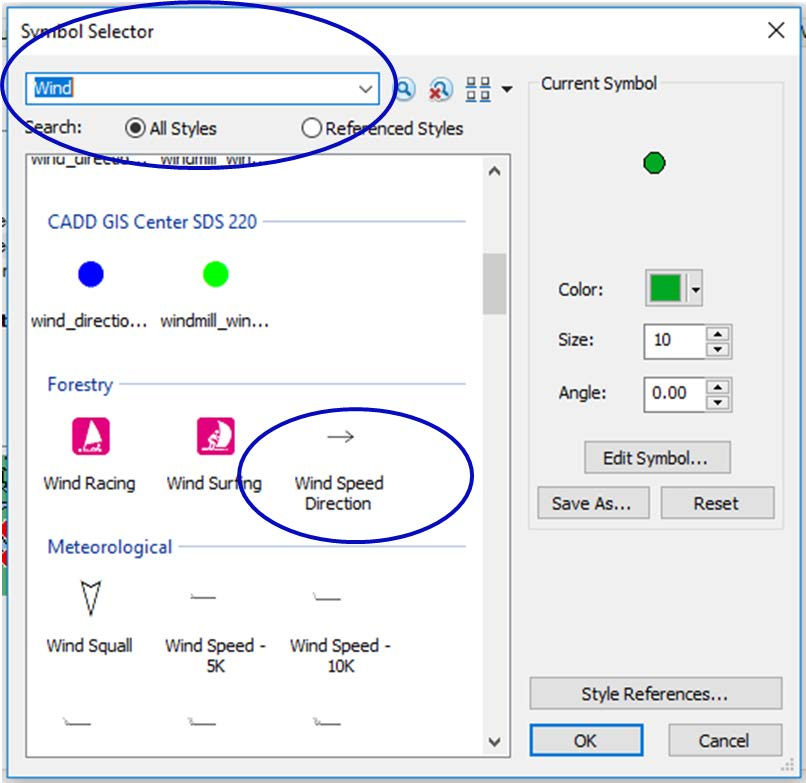
\includegraphics[scale=0.45]{arc_7.png}
    \caption{Warning Caption}
    \label{fig:Figure7}
\end{figure}

\item Select a symbol to represent the wind vectors (Figure ~\ref{fig:Figure8}). In the symbol \textbf{Gallery}, either search arrow or scroll down to find the arrow symbols under \textbf{ArcGIS Pro 2D}. Arrow markers \textbf{5}, \textbf{6}, and \textbf{20} are recommended.

\begin{figure}[H]
	\centering
	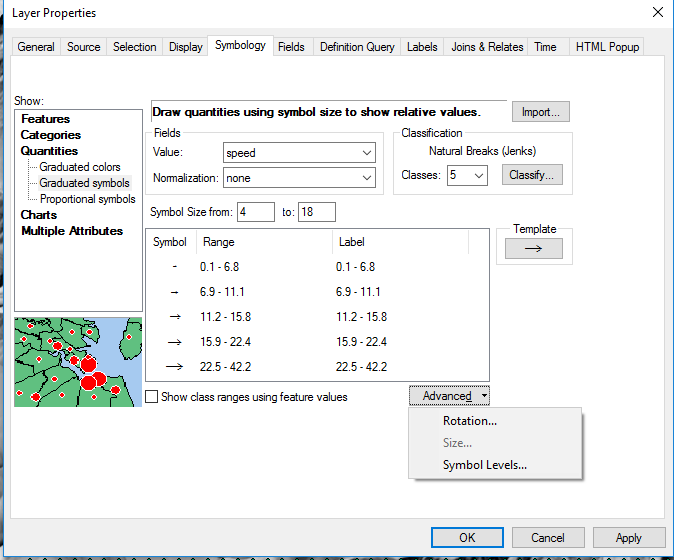
\includegraphics[scale=0.35]{arc_8.png}
	\caption{Select the template symbol to access available symbol sets.}
\label{fig:Figure8}
\end{figure}

\begin{figure}[H]
	\centering
	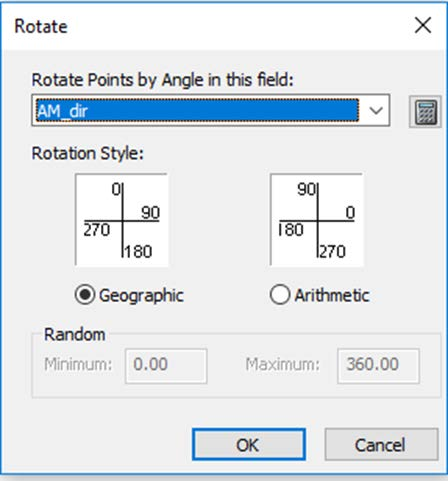
\includegraphics[scale=0.5]{arc_9.png}
	\caption{Symbol selector dialog box}
\label{fig:Figure9}
\end{figure}

\item Select an arrow symbol to represent the wind vectors, and the symbols on the map will be updated. Now return to the \textbf{Symbology Panel}.

\item Click on the \textbf{Vary Symbology By Attribute} tab, then click on \textbf{Rotation} which will open the \textbf{Rotation} drop down (Figure ~\ref{fig:Figure9}). In the drop down, select \textbf{AM\_dir} to rotate the points from the available options and select \textbf{Geographic} for \textbf{Rotation Style} (Figure ~\ref{fig:Figure10}).

\begin{figure}[H]
	\centering
	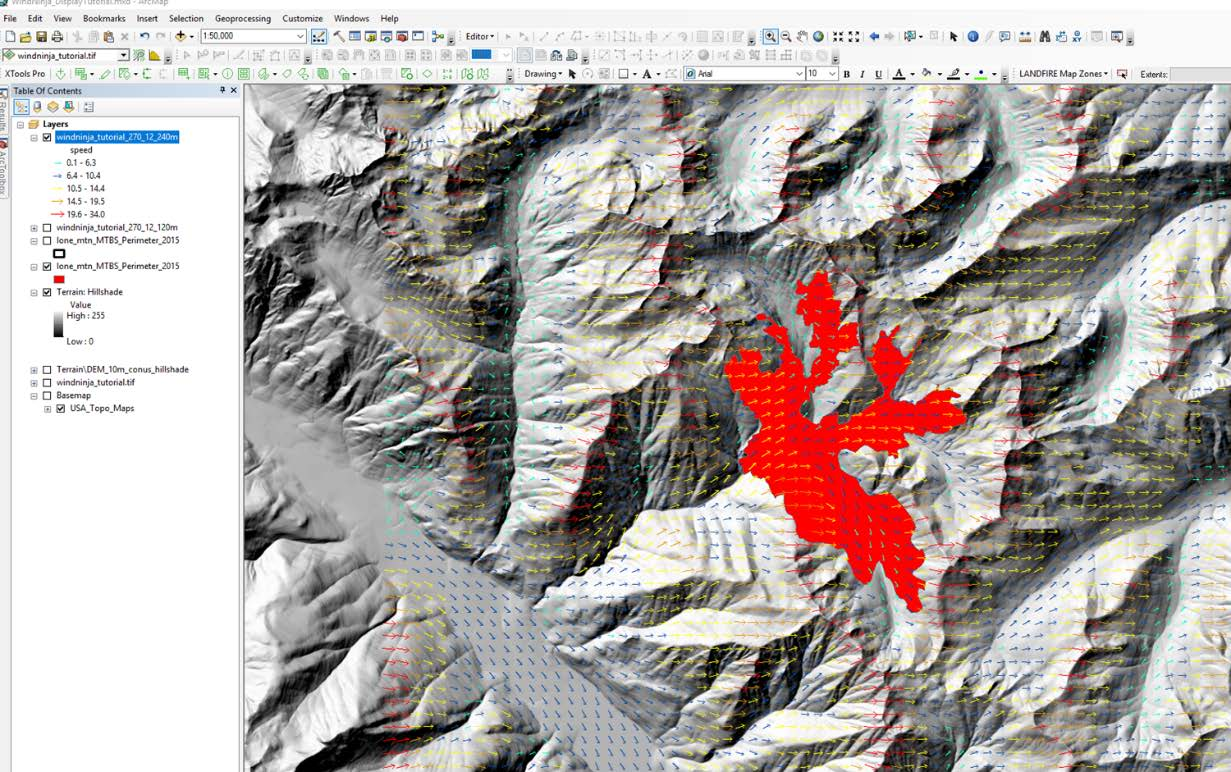
\includegraphics[scale=0.48]{arc_10.png}
	\caption{Selecting the Vary Symbology by Attribute and Rotation drop down.}
\label{fig:Figure10}
\end{figure}

\begin{figure}[H]
	\centering
	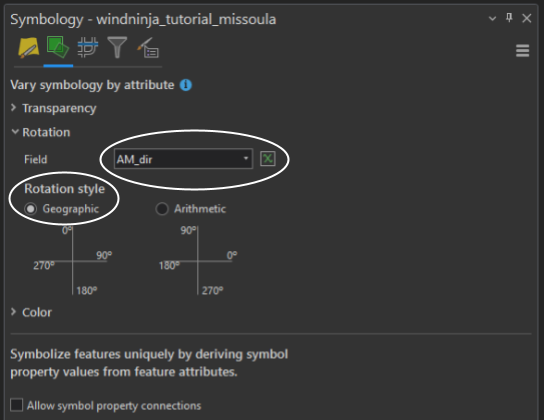
\includegraphics[scale=0.58]{arc_11.png}
	\caption{Rotation Field and style options.}
\label{fig:Figure11}
\end{figure}

\item \textbf{Optional:} Set a color ramp for the arrows based on wind speed by clicking the \textbf{Color} drop down. In the \textbf{Field} dropdown, select \textbf{speed} and select a \textbf{Color scheme} (Figure~\ref{fig:Figure12}).

\begin{figure}[H]
	\centering
	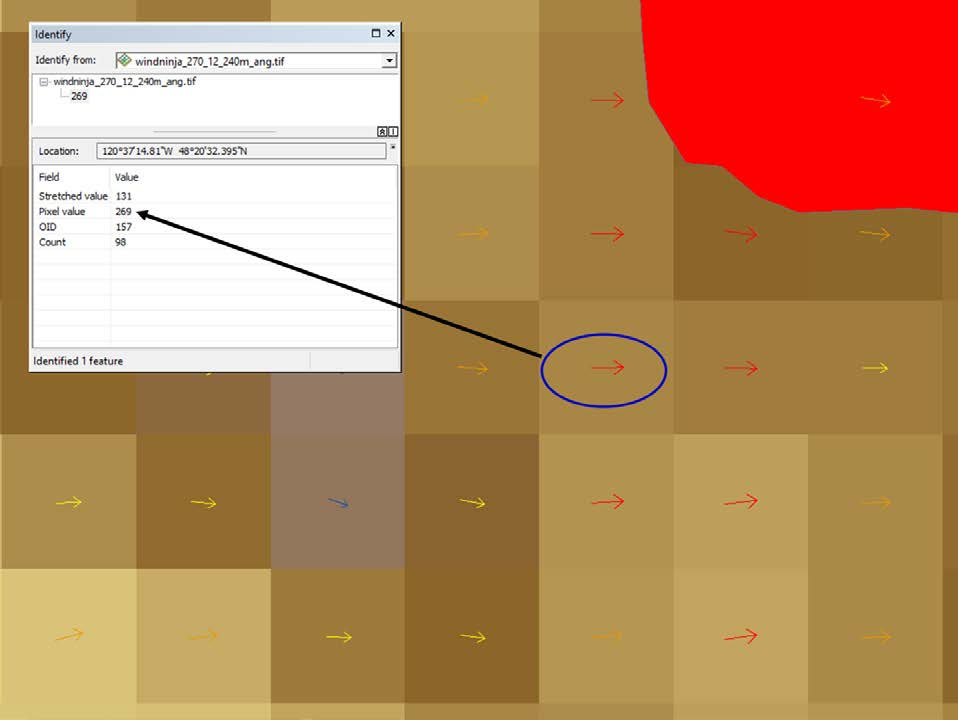
\includegraphics[scale=0.55]{arc_12.png}
	\caption{Color dialog box options.}
\label{fig:Figure12}
\end{figure}

\item You can now exit the \textbf{Symbology} panel.

\item The wind vectors will appear over the existing layers (Figure~\ref{fig:Figure13})

\begin{figure}[H]
	\centering
	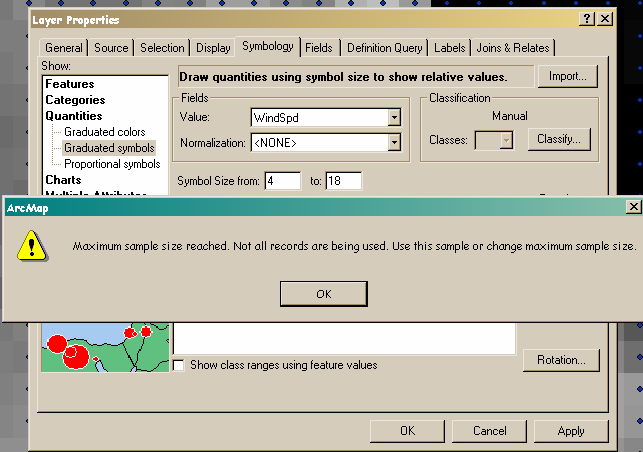
\includegraphics[scale=0.45]{arc_13.png}
	\caption{Rotated WindNinja vectors displayed in ArcGIS Pro.}
\label{fig:Figure13}
\end{figure}

\end{enumerate}

\section*{Query the Gridded Wind Output in ArcGIS Pro}
To correctly rotate the arrows in ArcGIS Pro as described above requires manipulation of the data generated by the WindNinja software for display purposes. In Figure~\ref{fig:Figure14}, the query information for the circled arrow shows the wind speed as 4.7 mph with an AM\_dir of 343. The AM\_dir value for wind direction in the shapefile \textbf{IS NOT} the same value as generated by the WindNinja software; it is for rotation and display purposes only. For this point, the wind speed is 4.7 mph (speed), and the wind is coming from 253 degrees (Dir). The values for speed and dir are the WindNinja-derived values that should be used in any analysis using this shapefile.

\textbf{Note}: The ASCII file output from WindNinja will have three separate files. There will be an filename\_ang.asc, filename\_cld.asc, and filename\_vel.asc which represent the wind direction, cloud cover percentage, and wind speed (velocity). 

\begin{figure}[H]
	\centering
	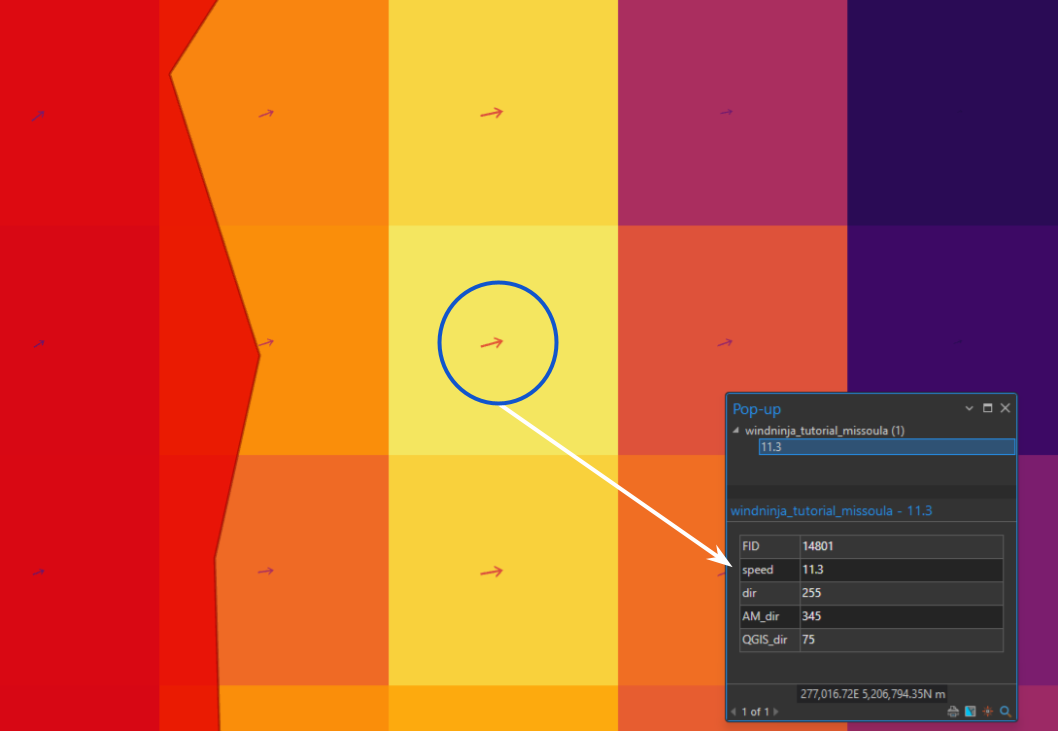
\includegraphics[scale=0.5]{arc_14.png}
	\caption{Query results of vector wind shapefile in ArcGIS Pro showing the difference in the wind direction in the shapefile and the rotation angle of the arrow. Query done after the shapefile has been rotated following previous steps.}
\label{fig:Figure14}
\end{figure}

\newpage

Figure~\ref{fig:Figure15} focuses on the same point on the landscape. However, in this case the ArcGIS Pro shapefile is
overlayed on the ASCII GRID of wind speed generated by the WindNinja software. A query of the individual
raster cell shows a pixel value of 4.72 which corresponds to the speed of the wind.
\begin{figure}[H]
	\centering
	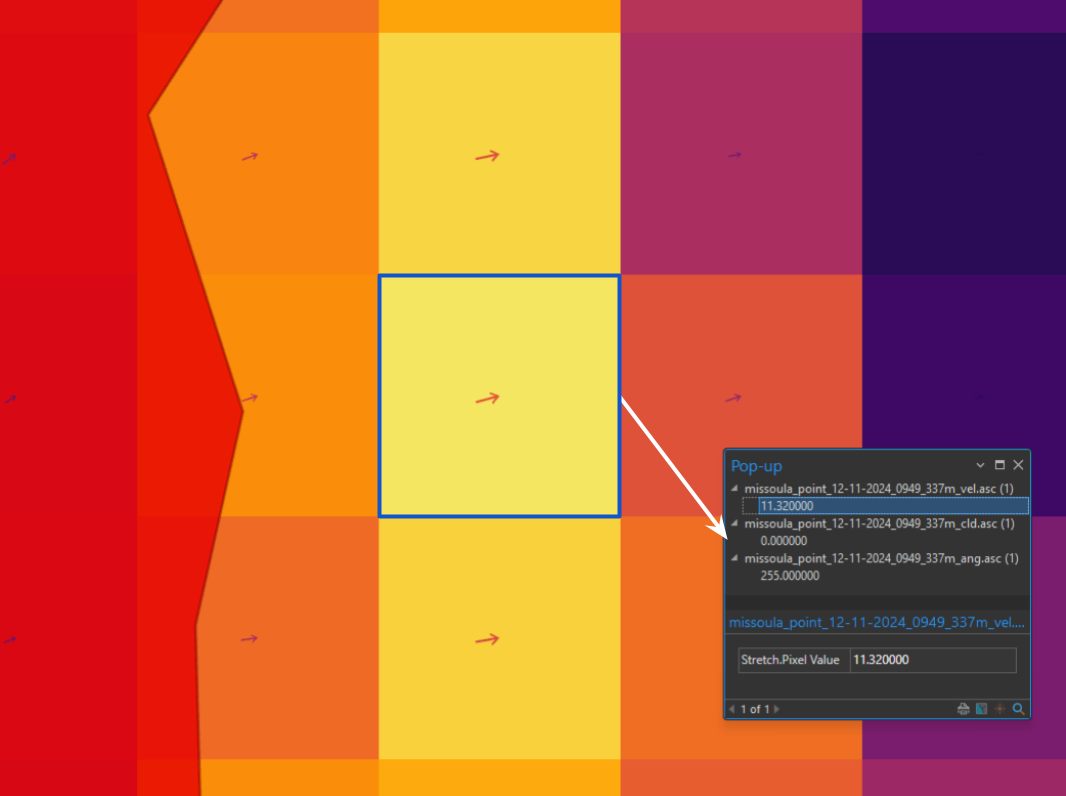
\includegraphics[scale=0.45]{arc_15.png}
	\caption{Query of the gridded wind raster generated ArcGIS Pro shapefile overlayed on the GRID ASCII Raster output from the WindNinja software.}
\label{fig:Figure15}
\end{figure}


\renewcommand{\thefigure}{\arabic{figure}}
\setcounter{figure}{0}

\pagebreak
\begin{centering}
\section*{Appendix}
\label{section:appendix}

\subsection*{How to Change the Number of Records Used In ArcGIS Pro when Displaying WindNinja Shapefile Output}
Gabriel Abreu Vigil, RMRS, Fire Sciences Lab, Missoula, MT, \href{mailto:gabriel.abreuvigil@usda.gov}{gabriel.abreuvigil@usda.gov}.
\end{centering}

When displaying the WindNinja-derived wind direction-speed shapefile information in ArcGIS Pro, the warning displayed in Figure~\ref{fig:Figure16} will often occur. This is because the default number of records to be displayed in ArcGIS Pro is the \textbf{First 10,000 Records} regardless of the distribution and spatial location of the data. Depending on the output file resolution size selected in the WindNinja software and the landscape extent, this number can easily be exceeded. As a consequence, not all records in the shapefile will be used during display of the wind speed values. Additionally, within ArcGIS Pro your choice of \textbf{Classification Method} and the number of \textbf{Classes} will also affect the displayed ranges of information.

\begin{figure}[H]
	\centering
	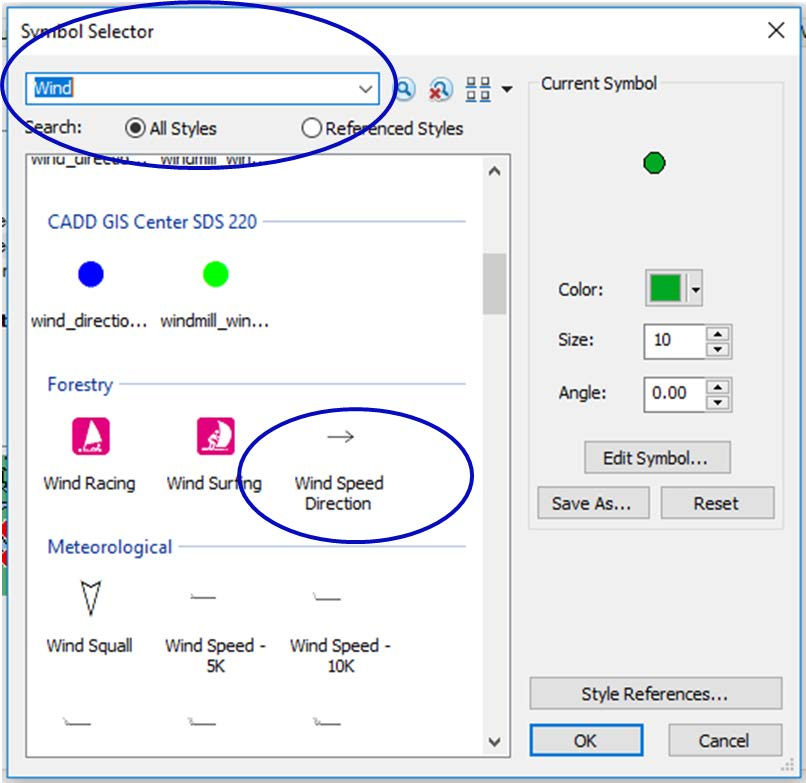
\includegraphics[scale=0.55]{arc_7.png}
	\caption{Error message when the number of records in the WindNinja ArcGIS Pro shapefile exceeds the default settings.}
\label{fig:Figure16}
\end{figure}

Because only the first 10,000 records are used, not all of the information will be used in defining the ranges of wind speed during the rotation process. This can lead to a misunderstanding of what the actual maximum and minimum wind speed values are. For example, in Figure~\ref{subfig:s16} the maximum wind speed value displayed is 7.3 mph while in Figure~\ref{subfig:s17} the maximum wind speed value displayed is 18.4 mph. These statistics are based on the total number of records used as limited by the Number of Records used.

\begin{figure}[H]
\centering
\subfloat[Using default setting
of 10,000 records]{
		  \label{subfig:s16}
		  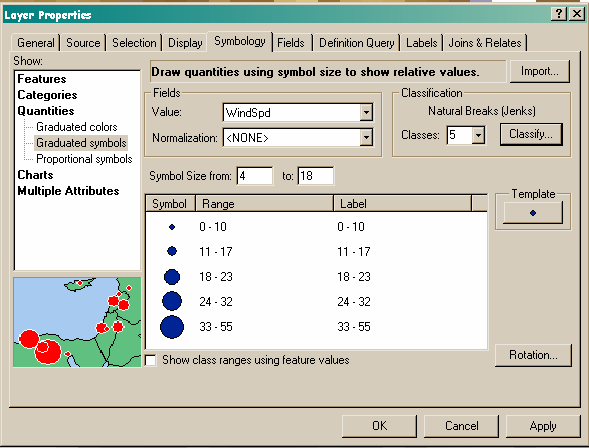
\includegraphics[scale=0.3]{arc_16.png}}\\
\subfloat[Setting Maximum Sample size so all records are used]{
		  \label{subfig:s17}
		  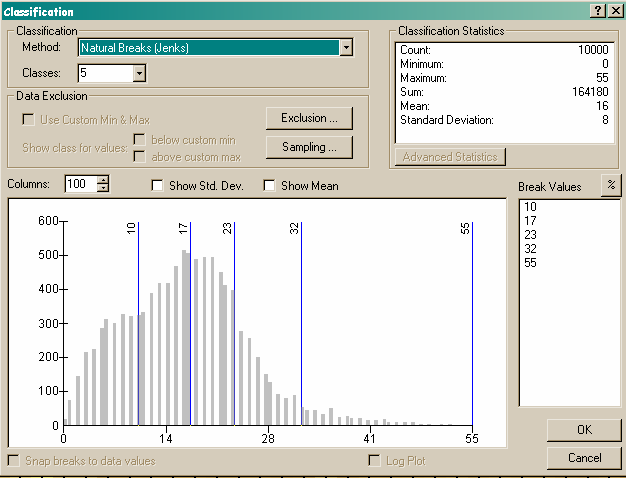
\includegraphics[scale=0.3]{arc_17.png}}
\caption{Displayed ranges of wind speed values based on Maximum Sample Size. (\ref{subfig:s16}) Using default setting of 10,000 records and (\ref{subfig:s17}) Setting Maximum Sample size so all records are used}
\label{fig:Figure17}
\end{figure}

\pagebreak

To change the number of records used for the shapefile is easy. This is not a universal change to the ArcGIS Pro settings but only applies to the shapefile while active in the view. Thus, every time you add this file to another ArcGIS Pro project you will have to repeat this step. To show the statistics, click on \textbf{More} and select \textbf{Show Statistics}. Then, select the \textbf{Histogram} tab next to the \textbf{Classes} tab. This will display the a graphical representation of the classes with their statistics, as seen in Figure ~\ref{fig:Figure18}.

\begin{figure}[H]
	\centering
	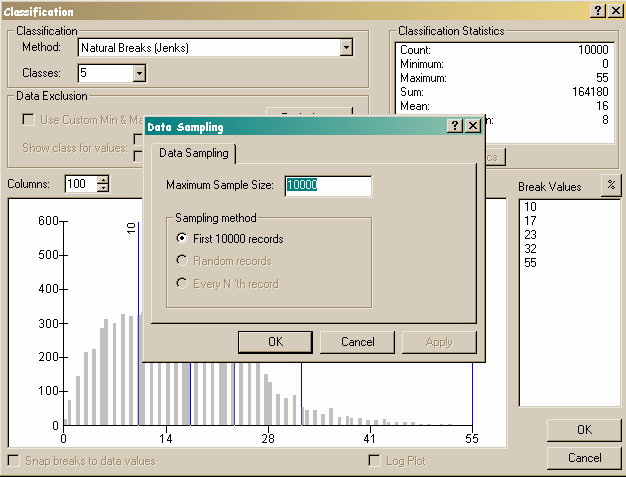
\includegraphics[scale=0.42]{arc_18.png}
	\caption{Histogram window with the statistics option selected as displayed in ArcGIS Pro.}
\label{fig:Figure18}
\end{figure}

In the \textbf{Statistics} table you can see the number of records used (Count), minimum and maximum, mean, and standard deviation. All of these values will change based on the Data Sampling method selected; in this case the number of values is the default value of first 10,000 records.  

\textbf{Note}: The number of records or sampling method chosen here does not affect summary or statistical operations performed on the data fields within the shapefile attribute table. Operations performed on the shapefile attribute table will use all of the records available for the selected data field unless a subset of the records has been selected. 

To change the \textbf{Maximum sampling size}, select the \textbf{Advanced Symbology Options} tab. This will open the window seen in Figure~\ref{fig:Figure19} where you will then click on the dropdown for \textbf{Sample size}. 

\begin{figure}[H]
	\centering
	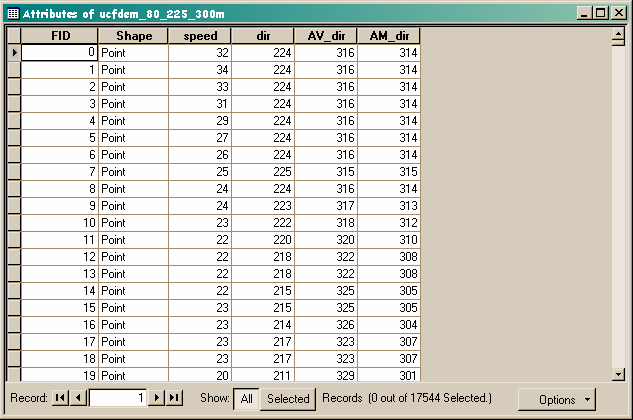
\includegraphics[scale=0.8]{arc_19.png}
	\caption{Input box for specifying the maximum sample size for the shapefile in ArcGIS Pro}
\label{fig:Figure19}
\end{figure}

You will need to change the \textbf{Maximum sample size} input used from 10,000 to a larger value (Figure~\ref{fig:Figure18}). After changing the \textbf{Maximum Sample Size}, exit the \textbf{Symbology} window and view the changes. For most shapefiles, changing this value to 100,000 should ensure that all records are being used. However, the number of records included in any one shapefile is determined by the size of the landscape as well as the output resolution selected in the WindNinja software. Because of this you may need to set this value higher in some cases.

To see how many records are in the shapefile, you can do the following.
\begin{enumerate}

\item In the \textbf{Table of Contents} pane right-click on the shapefile of interest.
\item  Select \textbf{Attribute Table}.
\item On the bottom of the window will be the statement “Records (0 out of \#\# Selected). The \#\# will be the total number of records in the shapefile (Figure~\ref{fig:Figure19}). If a subset of the total number of records has been selected this too can be determined. The number of selected records would show up where the 0 is for this example.
\end{enumerate}

\begin{figure}[H]
	\centering
	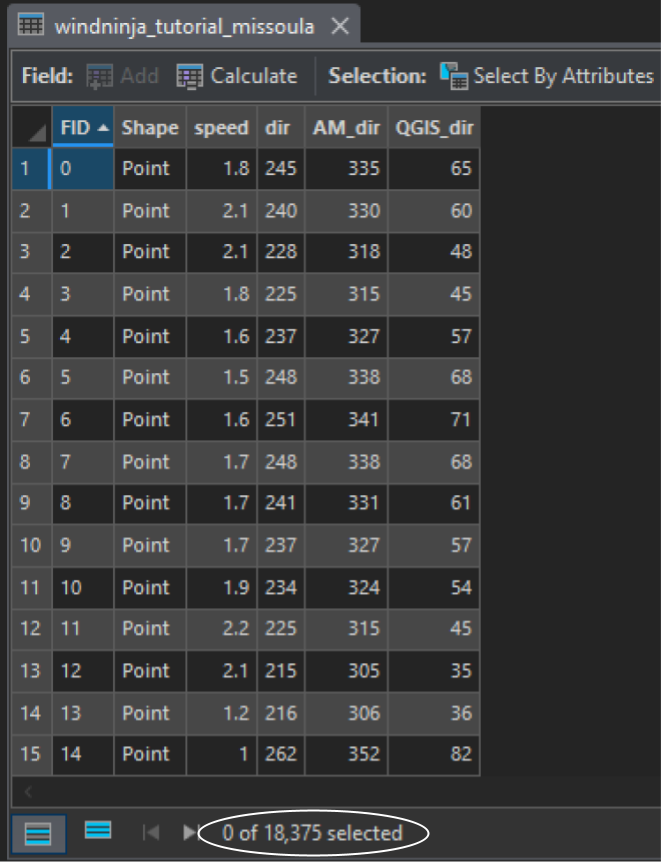
\includegraphics[scale=0.45]{arc_20.png}
	\caption{Attribute table for WindNinja-generated shapefile in ArcGIS Pro.}
\label{fig:Figure20}
\end{figure}

\end{document}